% ===========================================================================
% Informe final · Clustering the Star — Mercedes-Benz · III Malackathon 2026
% Compilación: pdflatex -> biber -> pdflatex -> pdflatex  (o latexmk -pdf, o Overleaf)
% ===========================================================================
\documentclass[11pt,a4paper]{article}

\usepackage[utf8]{inputenc}
\usepackage[T1]{fontenc}
\usepackage[spanish,es-tabla,es-nodecimaldot,es-noshorthands]{babel}
\usepackage{lmodern}
\usepackage{microtype}
\usepackage[a4paper,margin=2.5cm]{geometry}
\usepackage{graphicx}
\usepackage{booktabs}
\usepackage{tabularx}
\usepackage{array}
\usepackage{float}
\usepackage[font=small,labelfont=bf]{caption}
\usepackage{xcolor}
\usepackage{enumitem}
\usepackage{amsmath}
\usepackage[hidelinks]{hyperref}
\usepackage{csquotes}
\usepackage[backend=biber,style=authoryear,maxcitenames=2,maxbibnames=10,uniquelist=false]{biblatex}
\addbibresource{bibliografia.bib}

\graphicspath{{figuras/}}
\definecolor{petroleo}{HTML}{00677F}
\newcommand{\pct}{\,\%}
\newcommand{\seg}[1]{\textit{#1}}
\newcolumntype{L}{>{\raggedright\arraybackslash}X}
\setlist{itemsep=2pt,topsep=4pt}
\renewcommand{\arraystretch}{1.15}

\title{\textbf{Clustering the Star}\\[4pt]
\large Segmentación de clientes de Mercedes-Benz en Austria y Suiza\\[2pt]
\normalsize Informe final de los retos básicos y avanzados · III Malackathon 2026 · Universidad de Málaga}
\author{Equipo Mercedes-Benz · Malackathon 2026}
\date{}

\begin{document}
\maketitle

\begin{abstract}
\noindent Este informe recoge el trabajo completo sobre el reto \emph{Clustering the Star} de Mercedes-Benz: la
segmentación de 173.456 clientes de Austria y Suiza a partir de 302.850 relaciones cliente--vehículo. Tras una auditoría
de calidad del dato, se construye un \emph{pipeline} reproducible de doce variables por cliente y se entrena un modelo
K-Means con seis segmentos, a los que se da un nombre comercial y un plan de acción: \seg{Premium Multivehículo},
\seg{Fiel de Taller}, \seg{Pionero Eléctrico}, \seg{Gran Formato}, \seg{Recién Llegado de Ocasión} y
\seg{Contacto Solo Digital}. Los retos avanzados comparan K-Means con modelos de mezclas gaussianas, agrupamiento
jerárquico y DBSCAN; visualizan la estructura con análisis de componentes principales, y validan la estabilidad de los
segmentos con \emph{Jackknife Clustering}: el 99,1\pct\ de los clientes cae siempre en el mismo segmento aunque se
excluya un 20\pct\ de la base. Además, los datos internos se enriquecen con estadísticas oficiales de seguridad vial y
de salud (Statistik Austria, ASTRA, swisstopo, BAG y Eurostat), lo que permite detectar relaciones no evidentes, un
sesgo oculto en la variable de poder adquisitivo y nuevas oportunidades comerciales relacionadas con la seguridad y la
ergonomía.
\end{abstract}

\tableofcontents
\newpage

% ===========================================================================
\section{Introducción}
% ===========================================================================

\subsection{Contexto}

Mercedes-Benz dispone de una base de clientes conectados en Austria y Suiza con información sobre el perfil del
cliente (edad, género inferido, antigüedad como cliente, consentimientos de contacto), sus vehículos (clase, motorización,
fecha de matriculación, relación actual o pasada), su relación financiera (leasing), su uso del taller oficial, datos
socioeconómicos de su código postal y, para una parte de los vehículos, telemetría de conducción. El reto plantea
segmentar a estos clientes para que el equipo de marketing pueda diseñar ofertas de vehículos, planes de mantenimiento,
campañas de fidelización y comunicaciones dirigidas.

\subsection{Objetivos}

Los objetivos coinciden con los cuatro retos básicos y los tres avanzados del enunciado:
\begin{enumerate}
  \item \textbf{Reto 1 · Exploración y calidad del dato.} Entender la granularidad del fichero, auditar los valores nulos
        y las inconsistencias, y describir la base de clientes.
  \item \textbf{Reto 2 · Ingeniería de variables.} Seleccionar y construir las variables que describen a cada cliente y
        encapsular su preparación en un \emph{pipeline} reproducible.
  \item \textbf{Reto 3 · Modelo K-Means.} Elegir el número de segmentos con el método del codo y el coeficiente de
        silueta, y entrenar el modelo final.
  \item \textbf{Reto 4 · Interpretación.} Describir cada segmento en lenguaje de negocio, ponerle nombre y proponer
        acciones.
  \item \textbf{Avanzado 1 · Comparativa de algoritmos}, \textbf{Avanzado 2 · Reducción de dimensionalidad (PCA)} y
        \textbf{Avanzado 3 · Estabilidad con Jackknife Clustering}.
\end{enumerate}

A estos objetivos se ha añadido uno propio: \textbf{enriquecer la base con datos oficiales de salud y seguridad vial},
unidos por código postal o por edad y sexo, para buscar relaciones que los datos internos no muestran por sí solos.

\subsection{Estructura del informe}

La sección~\ref{sec:arte} resume el estado del arte; la sección~\ref{sec:metodo}, los datos y la metodología; la
sección~\ref{sec:resultados}, los resultados de cada reto con sus gráficos más relevantes; la
sección~\ref{sec:aclaraciones} aclara las decisiones que pueden generar dudas; y las secciones~\ref{sec:conclusiones}
y~\ref{sec:futuro} recogen las conclusiones y las líneas futuras. Todo el código está en el repositorio del equipo
(notebooks \texttt{Reto1\_EDA} a \texttt{Avanzado3\_Jackknife} y el módulo \texttt{features.py}), junto con un documento
explicativo de cada reto.

% ===========================================================================
\section{Estado del arte}\label{sec:arte}
% ===========================================================================

\subsection{Segmentación de clientes}

La segmentación de mercado parte de la idea de que una demanda heterogénea se atiende mejor dividiéndola en grupos
homogéneos con necesidades parecidas \parencite{smith1956}. \textcite{wedel2000} distinguen entre segmentaciones
\emph{a priori}, en las que el analista fija los criterios (por ejemplo, edad o renta), y \emph{post hoc}, en las que
los grupos se descubren a partir de los datos mediante técnicas de agrupamiento. Este trabajo es del segundo tipo: los
segmentos surgen del comportamiento del cliente (vehículos, financiación, taller, contacto) y no de una regla fijada de
antemano. Los mismos autores insisten en que un buen segmento debe ser \emph{identificable}, \emph{sustancial},
\emph{accesible}, \emph{estable} y \emph{accionable}; estos criterios guían la elección del número de segmentos
(sección~\ref{sec:r3}) y la validación de estabilidad (sección~\ref{sec:a3}).

\subsection{K-Means y sus alternativas}

K-Means \parencite{macqueen1967,lloyd1982} divide las observaciones en $k$ grupos minimizando la suma de distancias
cuadráticas de cada punto al centroide de su grupo (la \emph{inercia}). Es el algoritmo de agrupamiento más utilizado por
su sencillez, su escalabilidad y la interpretabilidad de sus centroides \parencite{jain2010,steinley2006}. Sus
limitaciones son conocidas: asume grupos aproximadamente esféricos y de varianza parecida, depende de la escala de las
variables y converge a óptimos locales, por lo que se ejecuta con varias inicializaciones; la inicialización
\emph{k-means++} \parencite{arthur2007} reduce este problema.

Entre las alternativas habituales destacan los modelos de mezclas gaussianas (GMM), que estiman cada grupo como una
distribución normal mediante el algoritmo EM \parencite{dempster1977} y permiten grupos de distinta forma y una
asignación probabilística; el agrupamiento jerárquico aglomerativo, en particular con el criterio de \textcite{ward1963},
que comparte con K-Means la minimización de la varianza intragrupo; y DBSCAN \parencite{ester1996}, que define los
grupos como regiones densas separadas por zonas vacías y no requiere fijar $k$.

\subsection{Selección del número de grupos y validación}

No existe un criterio único para elegir $k$. El método del codo \parencite{thorndike1953} busca el punto a partir del
cual añadir grupos apenas reduce la inercia; el coeficiente de silueta \parencite{rousseeuw1987,kaufman1990} compara, para cada
observación, la distancia media a su grupo con la distancia media al grupo vecino más cercano; los índices de
\textcite{calinski1974} y \textcite{davies1979} relacionan la dispersión entre grupos con la dispersión interna; y el
estadístico \emph{gap} \parencite{tibshirani2001} compara la inercia con la esperada en datos sin estructura. Todos estos
criterios son internos y basados en distancias euclídeas, por lo que tienden a favorecer soluciones compactas y
esféricas \parencite{hastie2009}. En segmentación comercial, la literatura recomienda combinarlos con criterios de
negocio \parencite{wedel2000}. Para comparar dos particiones se usa el índice de Rand ajustado (ARI) de
\textcite{hubert1985}, que no depende de cómo se numeren los grupos; cuando hace falta emparejar grupos entre dos
soluciones, el algoritmo húngaro \parencite{kuhn1955} encuentra la correspondencia óptima.

\subsection{Estabilidad de los agrupamientos}

Un agrupamiento puede obtener buenas métricas internas y, aun así, cambiar mucho ante pequeñas variaciones de los
datos. Las técnicas de remuestreo, como el \emph{jackknife} \parencite{quenouille1949} y el \emph{bootstrap}
\parencite{efron1979}, permiten medirlo: se re-entrena el modelo sobre submuestras y se compara la coherencia de las
asignaciones \parencite{benhur2002,lange2004,vonluxburg2010}. \textcite{hennig2007} propone medir la estabilidad
\emph{por grupo} con el índice de Jaccard entre cada grupo original y su mejor equivalente en cada remuestreo, con una
escala orientativa: por encima de 0,85, muy estable; por debajo de 0,5, el grupo se disuelve.

\subsection{Reducción de dimensionalidad}

El análisis de componentes principales \parencite{pearson1901,jolliffe2016} proyecta los datos sobre direcciones
ortogonales que recogen la máxima varianza. Es la herramienta habitual para visualizar agrupamientos en dos o tres
dimensiones, con una advertencia: si la varianza está repartida entre muchas componentes, el plano de las dos primeras
puede ocultar separaciones que existen en el espacio completo.

\subsection{Enriquecimiento con datos externos}

Unir datos de clientes con estadísticas territoriales (renta, siniestralidad, salud) por código postal es una práctica
extendida en geomarketing. Su principal riesgo es la \emph{falacia ecológica} \parencite{robinson1950}: una correlación
entre zonas no implica la misma relación entre las personas que viven en ellas. A esto se suma el marco legal: los
datos de salud son una categoría especial de datos personales \parencite{rgpd2016}, por lo que cualquier uso debe
limitarse a estimaciones agregadas, sin atribuir condiciones a individuos. En el ámbito del vehículo, la literatura
muestra que el consumo real de los híbridos enchufables es muy superior al homologado cuando se cargan poco
\parencite{plotz2021}, y que la exposición prolongada a la conducción y a las vibraciones se asocia con el dolor lumbar
\parencite{bovenzi1999}; ambos resultados se usan como contexto en la sección~\ref{sec:r1}.

% ===========================================================================
\section{Datos y metodología}\label{sec:metodo}
% ===========================================================================

\subsection{Datos del reto}

El fichero contiene 302.850 filas y 39 columnas. Cada fila es una \textbf{relación cliente--vehículo}: un cliente puede
tener varios vehículos (actuales o pasados) y un vehículo puede estar vinculado a varios clientes (propietario,
conductor, usuario temporal). Hay 173.456 clientes únicos (66,2\pct\ en Suiza y 33,8\pct\ en Austria) y 244.519
vehículos. Los atributos de cliente son constantes entre sus filas, pero la telemetría y las visitas al taller varían
entre clientes que comparten vehículo: son datos de la relación, no del vehículo.

\subsection{Principios metodológicos}

Todo el trabajo se rige por cinco principios:
\begin{enumerate}
  \item \textbf{Un cliente, una fila.} La segmentación es de clientes, así que todo se agrega a nivel de cliente; si no,
        los clientes con muchos vehículos pesarían más.
  \item \textbf{El país no segmenta.} Suiza y Austria tienen niveles de renta y prácticas de registro distintos. Las
        variables que dependen del país se expresan como \textbf{percentil dentro de su país}.
  \item \textbf{Cada decisión de limpieza se mide.} Antes de imputar o eliminar se comparan alternativas y su efecto
        sobre la base.
  \item \textbf{Cada hallazgo se enfrenta a su explicación aburrida} (edad del coche, país, ruralidad, poder
        adquisitivo) antes de darlo por bueno.
  \item \textbf{Reproducibilidad.} La preparación está en un \emph{pipeline} de scikit-learn \parencite{pedregosa2011}
        definido en \texttt{features.py}, con semilla y número de inicializaciones fijos.
\end{enumerate}

\subsection{Herramientas}

Python 3 con pandas \parencite{mckinney2010}, scikit-learn \parencite{pedregosa2011}, SciPy, Matplotlib
\parencite{hunter2007} y seaborn \parencite{waskom2021}. Los notebooks se generan y ejecutan de principio a fin para
garantizar que cada cifra del texto procede de una ejecución real.

\subsection{Datos externos}

Se han usado diez fuentes oficiales, todas documentadas con su organismo, dataset, enlace, periodo y condiciones de uso
en el fichero \texttt{Fuentes\_Datos\_Externos.md} del repositorio:
\begin{itemize}
  \item \textbf{Seguridad vial y salud por zona:} accidentes con heridos y su gravedad por distrito
        \parencite{statat2025}, mortalidad estandarizada por edad \parencite{statatmort}, municipios y códigos postales
        \parencite{statatgem} y hospitales \parencite{bmsgpk2026} en Austria; accidentes geolocalizados
        \parencite{astra2026}, localidades \parencite{swisstopo2026} y hospitales \parencite{bag2023} en Suiza. Se unen
        a cada cliente por país y código postal.
  \item \textbf{Salud por edad y sexo:} limitación en las actividades por motivos de salud (EU-SILC 2023, Austria y
        Suiza; \cite{eurostatsilc}) y problemas lumbares, cervicales y artrosis (EHIS 2019, solo Austria;
        \cite{eurostatehis}). Se asignan a cada cliente según su país, edad y sexo.
\end{itemize}
Los indicadores externos \textbf{no entran en el modelo}: se usan para entender los datos y perfilar los segmentos
(sección~\ref{sec:aclaraciones}).

% ===========================================================================
\section{Resultados por reto}\label{sec:resultados}
% ===========================================================================

\subsection{Reto 1 · Exploración y calidad del dato}\label{sec:r1}

\paragraph{Valores nulos.} La figura~\ref{fig:nulos} muestra el porcentaje de nulos por columna. La telemetría falta en
el 57--61\pct\ de las filas, la motorización en el 44\pct, el género en el 11\pct\ de las filas (17\pct\ de los
clientes) y las variables socioeconómicas en el 6,3\pct. El análisis del \emph{mecanismo} de cada nulo
\parencite{little2019} fue decisivo (figura~\ref{fig:mecanismo}): la telemetría no falta al azar, sino de forma
\textbf{estructural} (en el 100\pct\ de los eléctricos, en casi todos los roles no propietarios y en los coches
anteriores a 2016); la motorización depende del año del sistema de origen; y el género desconocido se concentra en los
clientes más jóvenes y en los mayores.

\begin{figure}[H]
  \centering
  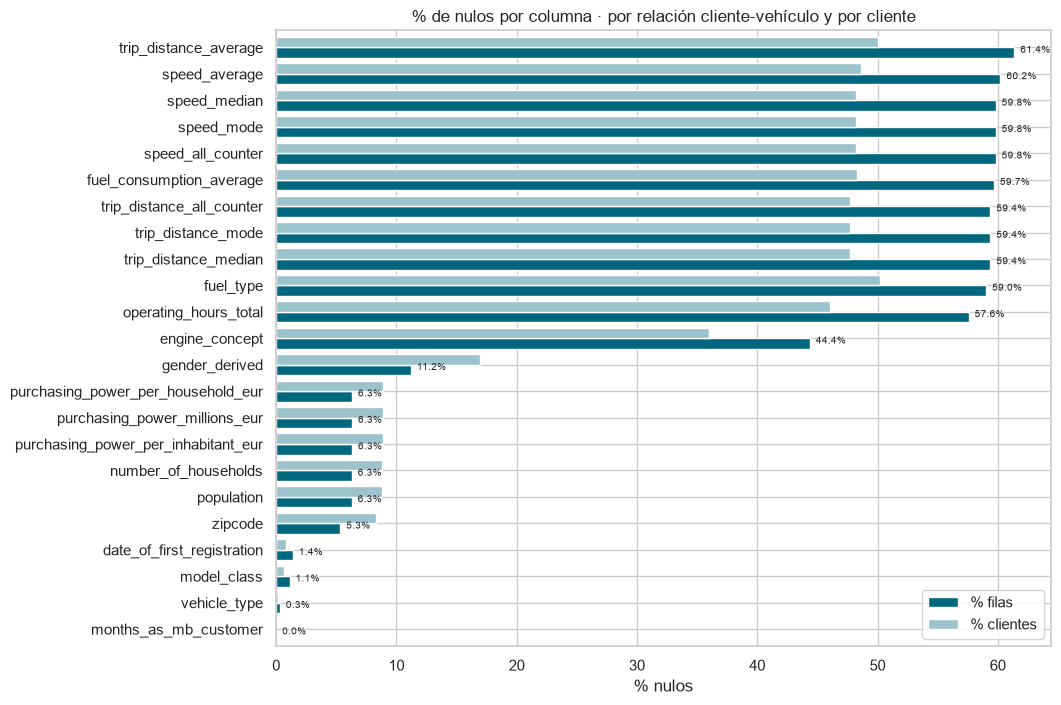
\includegraphics[width=0.85\textwidth]{r1_nulos.png}
  \caption{Porcentaje de nulos por columna, por relación cliente--vehículo y por cliente.}
  \label{fig:nulos}
\end{figure}

\begin{figure}[H]
  \centering
  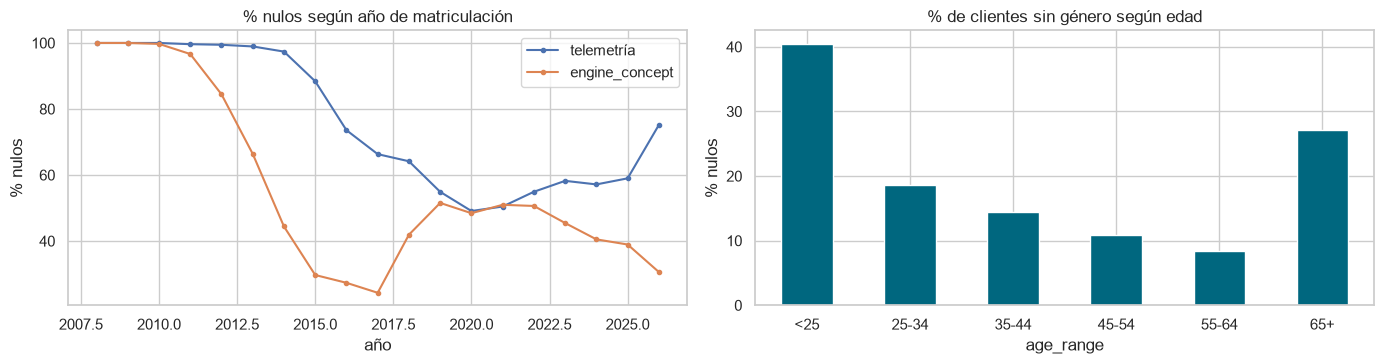
\includegraphics[width=0.95\textwidth]{r1_mecanismo_nulos.png}
  \caption{Mecanismo de los nulos: según el año de matriculación (izquierda) y según la edad del cliente (derecha).}
  \label{fig:mecanismo}
\end{figure}

\paragraph{Decisiones de imputación.} Eliminar los clientes con nulos habría supuesto perder el 18,6\pct\ de la base y
sesgarla (menos jóvenes, menos mayores y menos austriacos), por lo que se descartó. El poder adquisitivo se imputa con la
\textbf{mediana de su país}: la media global (47.189~€ por habitante) situaría a un austriaco sin dato por encima del
88\pct\ de su país. La telemetría ni se imputa ni entra en el modelo. El género se trata como categoría
\emph{desconocido} y queda fuera del modelo.

\paragraph{Inconsistencias.} Se detectaron medianas y modas de la telemetría que en realidad son límites de tramo de
un histograma, un pico artificial de clientes con exactamente 36 meses de antigüedad, códigos postales con formato
válido pero inexistentes (\texttt{0000}, \texttt{9999}) y una diferencia de \textbf{registro} de las visitas en garantía
entre países: con coches de antigüedad parecida, el 52\pct\ de los austriacos figura con cero visitas frente al 23\pct\
de los suizos. Por eso las visitas se expresan como percentil dentro del país. La figura~\ref{fig:taller} muestra además
que las visitas dependen de la edad del coche, lo que obliga a interpretarlas comparando coches de la misma antigüedad.

\begin{figure}[H]
  \centering
  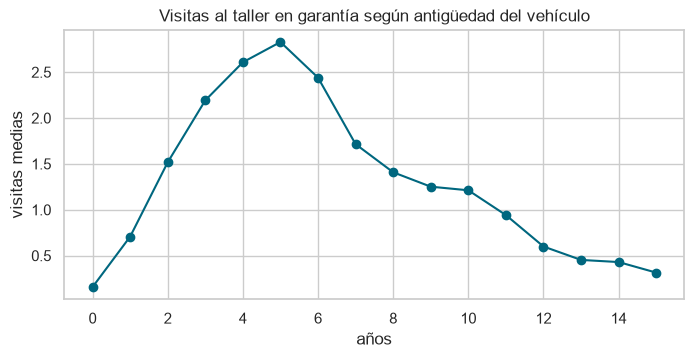
\includegraphics[width=0.6\textwidth]{r1_taller_antiguedad.png}
  \caption{Visitas en garantía según la antigüedad del vehículo: crecen hasta los cinco años y caen al terminar la
           garantía.}
  \label{fig:taller}
\end{figure}

\paragraph{Perfil de la base.} Clientela madura (60,8\pct\ con 45 años o más), mayoritariamente masculina según el
género inferido (65\pct), con una relación reciente (mediana de 36 meses), casi siempre con un único vehículo conectado
(el 10,4\pct\ no tiene ninguno), un 29,4\pct\ que ha usado alguna vez la financiación o el leasing (mucho más en Suiza),
uno de cada cuatro vehículos electrificados (más en Austria) y un consentimiento de email casi universal (98,3\pct).

\paragraph{Relaciones no evidentes dentro del CSV.} Se buscaron relaciones que cambien la interpretación o la oferta,
siempre controlando por la explicación más sencilla:
\begin{itemize}
  \item \textbf{Mayores con coche antiguo, pero poco usado} (figura~\ref{fig:mayores}). Los clientes de 65 años o más
        tienen el doble de coches de diez o más años (7,7\pct\ frente a $\approx$4\pct), pero, comparando coches de la
        misma edad, acumulan en torno a un 20\pct\ menos de horas de motor. Un coche antiguo con pocos kilómetros tiene un
        valor de recompra atractivo y su cambio natural es hacia un coche más seguro, no más caro.
  \item \textbf{Híbridos enchufables que no se cargan} (figura~\ref{fig:phev}). El consumo mediano de los PHEV es de
        5,8~L/100~km, lejos de los valores homologados, y uno de cada siete consume como un coche de combustión, en línea
        con \textcite{plotz2021}. Es un público para soluciones de carga y para el paso al 100\pct\ eléctrico.
  \item \textbf{El eléctrico entra como coche principal}: en los hogares con varios coches, el electrificado es el más
        nuevo (mediana de 1,5 años frente a 3,5) y de mayor gama.
  \item \textbf{El taller predice la permanencia}: con coches de la misma edad, los clientes sin visitas al taller
        oficial están inactivos entre 1,2 y 4,5 veces más. En cambio, el número de consentimientos no tiene relación con
        el abandono.
  \item \textbf{Otras ideas que se desmontan}: los AMG no se conducen más rápido que el resto (es un producto de
        imagen); el género desconocido indica un perfil incompleto (clientes con la mitad de antigüedad); y la riqueza de
        la zona apenas cambia la gama elegida.
\end{itemize}

\begin{figure}[H]
  \centering
  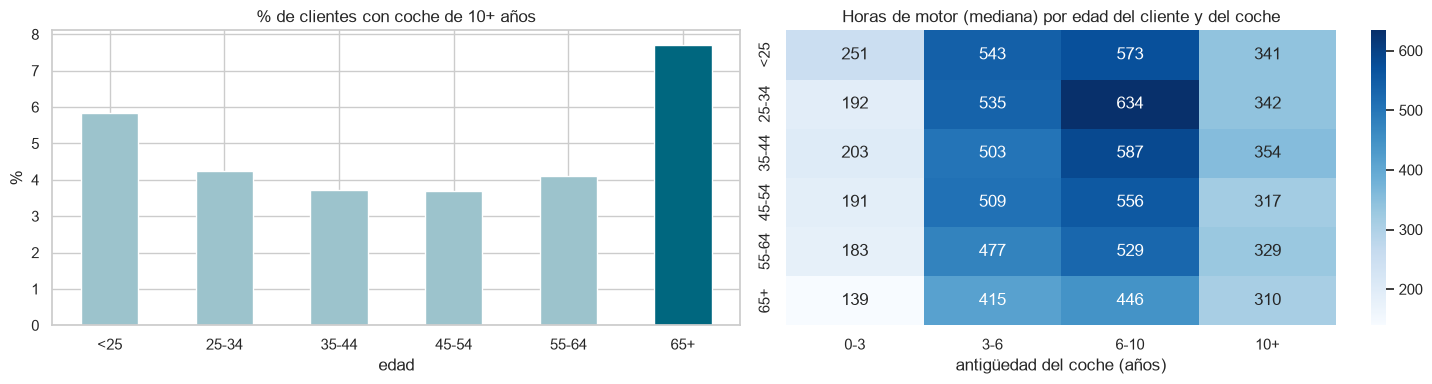
\includegraphics[width=\textwidth]{r1_mayores_coche.png}
  \caption{Porcentaje de clientes con coche de diez o más años por edad (izquierda) y horas de motor según la edad del
           cliente y del coche (derecha). Las horas son un contador acumulado, por lo que solo se comparan coches de la
           misma antigüedad.}
  \label{fig:mayores}
\end{figure}

\begin{figure}[H]
  \centering
  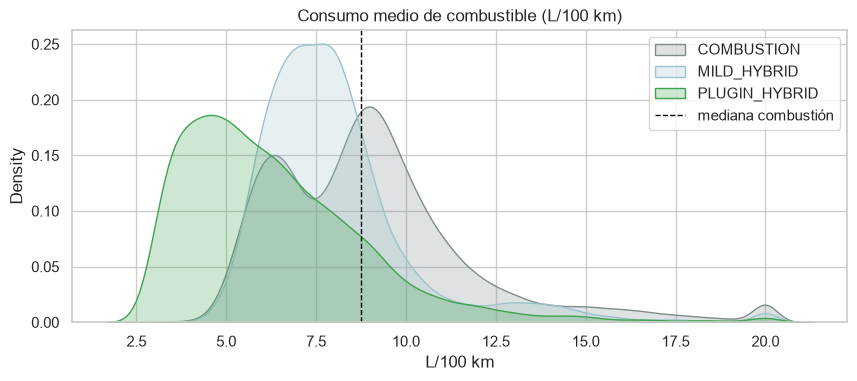
\includegraphics[width=0.7\textwidth]{r1_phev.png}
  \caption{Consumo medio por motorización. Una parte de los híbridos enchufables consume como un coche de combustión.}
  \label{fig:phev}
\end{figure}

\paragraph{Relaciones con los datos de seguridad vial.} Al cruzar la base con los indicadores de zona apareció un
\textbf{problema de calidad}: en Austria, las zonas rurales parecían más ricas. La causa es que el poder adquisitivo
\emph{por hogar} crece con el tamaño del hogar (correlación de Spearman \parencite{spearman1904} de +0,67 con las
personas por hogar), mientras que el \emph{por habitante} no tiene relación con la ruralidad ($-0{,}03$ con la distancia
al hospital). El modelo pasó a usar el poder adquisitivo por habitante. La figura~\ref{fig:parciales} muestra las
correlaciones parciales entre zonas, descontando poder adquisitivo y ruralidad:
\begin{itemize}
  \item La \textbf{telemetría valida los datos externos}: en los distritos con más accidentes graves, los clientes
        conducen más rápido (de 43 a 55~km/h de media entre el primer y el último cuartil).
  \item Las zonas con más accidentes \textbf{no tienen coches más viejos, sino más nuevos}, con más leasing y más
        vehículos que el cliente ya no conserva, lo que sugiere un programa de retención \emph{posterior al siniestro}.
  \item En los distritos con \textbf{más mortalidad} hay coches más viejos y más clientes que nunca visitan el taller
        oficial, también con coches de la misma edad: una posible \emph{cultura de prevención} común a la salud y al
        coche.
  \item En Suiza solo aparecen relaciones débiles ($|\rho| \le 0{,}23$), coherentes con la menor variabilidad entre
        municipios.
\end{itemize}

\begin{figure}[H]
  \centering
  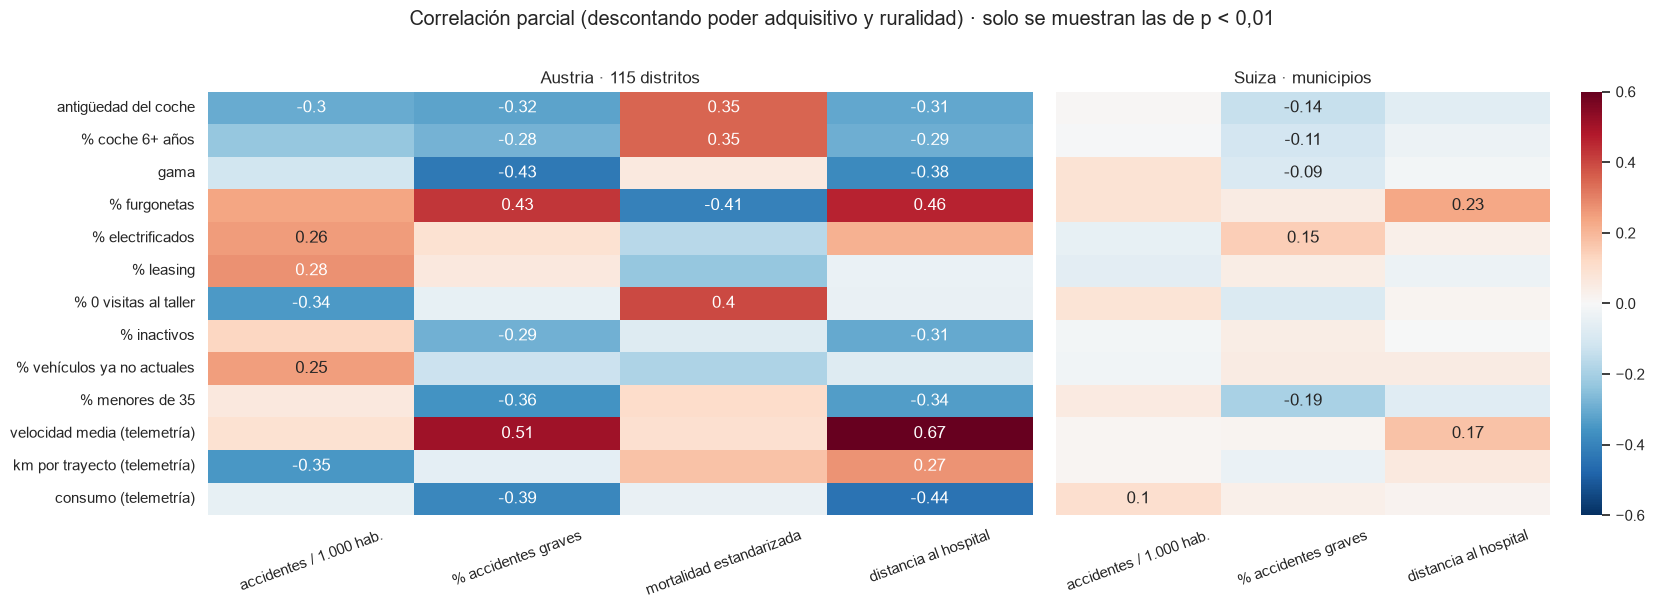
\includegraphics[width=\textwidth]{r1_correlaciones_parciales.png}
  \caption{Correlación parcial de Spearman entre los indicadores de zona y el perfil de los clientes, descontando poder
           adquisitivo y ruralidad. Solo se muestran los valores con $p<0{,}01$.}
  \label{fig:parciales}
\end{figure}

\paragraph{Salud y ergonomía.} Con las prevalencias oficiales por país, edad y sexo (figura~\ref{fig:eurostat}) se
estima, para cada cliente, la probabilidad \emph{esperada} de tener un problema de salud que afecte a la conducción. Se
esperan unos 55.000 clientes con alguna limitación por salud y, solo en Austria, unos 16.000 con problemas lumbares,
11.000 cervicales y 8.000 con artrosis. La figura~\ref{fig:brecha} muestra una \textbf{brecha ergonómica}: la limitación
esperada se duplica entre los 35--44 años y los mayores de 65 (del 22\pct\ al 48\pct), pero la proporción de coches de
posición alta (SUV, monovolumen, furgoneta), más fáciles de usar, se estanca en torno al 63\pct. Hay unos 12.400 clientes
de 65 años o más sin ningún coche alto, unos 5.900 de ellos con una limitación probable. Los conductores de furgoneta,
por su parte, hacen los trayectos más largos, un factor de riesgo de dolor lumbar \parencite{bovenzi1999}.

\begin{figure}[H]
  \centering
  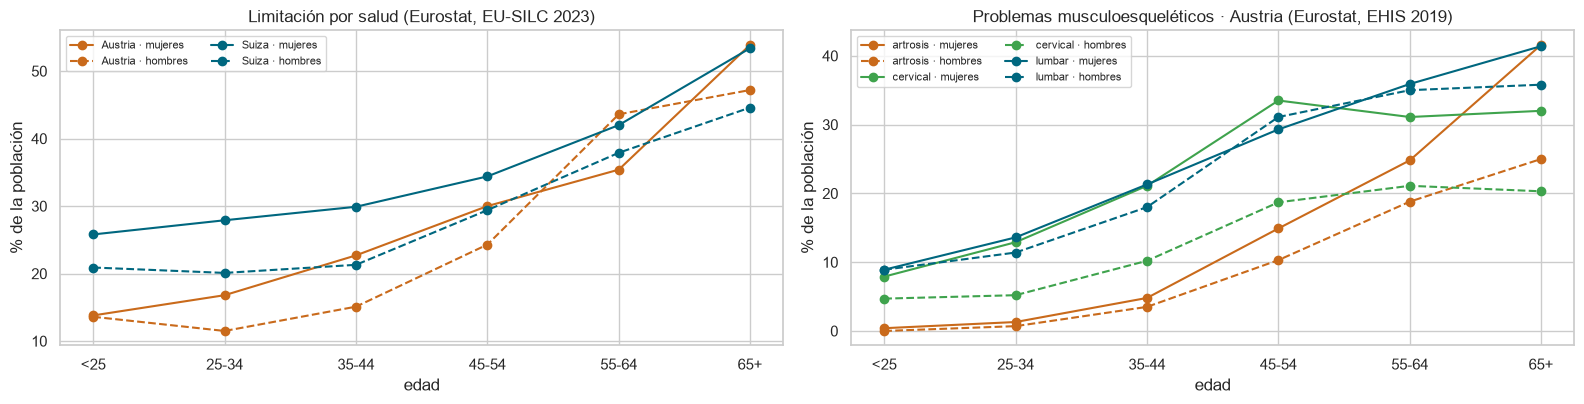
\includegraphics[width=\textwidth]{r1_salud_eurostat.png}
  \caption{Prevalencias oficiales por edad y sexo: limitación por salud en Austria y Suiza (izquierda) y problemas
           musculoesqueléticos en Austria (derecha). Fuentes: \textcite{eurostatsilc,eurostatehis}.}
  \label{fig:eurostat}
\end{figure}

\begin{figure}[H]
  \centering
  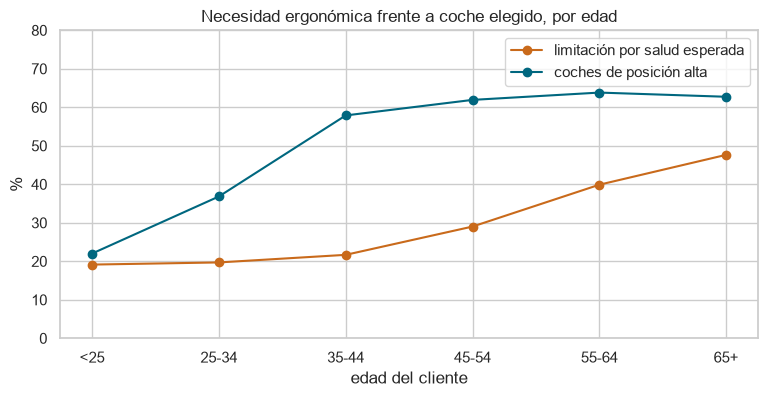
\includegraphics[width=0.7\textwidth]{r1_brecha_ergonomica.png}
  \caption{Limitación por salud esperada frente a la proporción de coches de posición alta, por edad del cliente.}
  \label{fig:brecha}
\end{figure}

\subsection{Reto 2 · Ingeniería de variables}\label{sec:r2}

Se definieron doce variables por cliente, ocho de ellas derivadas (tabla~\ref{tab:features}). La preparación se
encapsula en un \emph{pipeline} de tres pasos: agregación a una fila por cliente (incluida la unión con los datos
externos como columnas de perfilado), recorte de extremos (topes de 10 vehículos en el histórico, 5 actuales, 20 años de
antigüedad y 120 meses de relación) y un \texttt{ColumnTransformer} con imputación, codificación ordinal, transformación
logarítmica de los recuentos y escalado estándar.

\begin{table}[H]
  \centering
  \small
  \caption{Variables del modelo.}
  \label{tab:features}
  \begin{tabularx}{\textwidth}{lL}
    \toprule
    Variable & Qué mide y tratamiento \\
    \midrule
    Edad (tramo) & Etapa vital; ordinal \\
    Financiación / leasing & Nunca $\rightarrow$ antes $\rightarrow$ leasing $\rightarrow$ leasing y contado; ordinal \\
    Vehículos en el histórico$^\ast$ & Fidelidad acumulada; tope 10 y logaritmo \\
    Vehículos actuales & Tamaño de la relación hoy; tope 5 y logaritmo \\
    Meses como cliente & Antigüedad de la relación; tope 120 \\
    Antigüedad del vehículo$^\ast$ & Proximidad a la renovación; tope 20 años \\
    Gama máxima$^\ast$ & Nivel 1--4 de la clase más alta que ha tenido \\
    \% electrificado$^\ast$ & Afinidad con la electrificación (motor o, si falta, nombre comercial) \\
    \% furgoneta$^\ast$ & Uso profesional o familiar grande \\
    Canales consentidos$^\ast$ & Teléfono + email + correo postal \\
    Poder adquisitivo$^\ast$ & Percentil \emph{por habitante} dentro de su país; nulo $\rightarrow$ 0,5 \\
    Visitas al taller$^\ast$ & Percentil de visitas por vehículo dentro de su país \\
    \bottomrule
    \multicolumn{2}{l}{\footnotesize $^\ast$ Variable derivada.}
  \end{tabularx}
\end{table}

Quedaron fuera del modelo, y se usan solo para perfilar, el país, el género inferido, la relación B2B (1,8\pct\ de las
relaciones), la telemetría, los consentimientos por separado, las variables de modelo de alta cardinalidad y los
indicadores externos. La figura~\ref{fig:percentil} justifica el uso de percentiles: en euros, las poblaciones de Austria
y Suiza apenas se solapan; en percentil, la variable deja de distinguir países. Ninguna pareja de variables está
fuertemente correlacionada (máximo 0,52, entre meses como cliente y visitas al taller).

\begin{figure}[H]
  \centering
  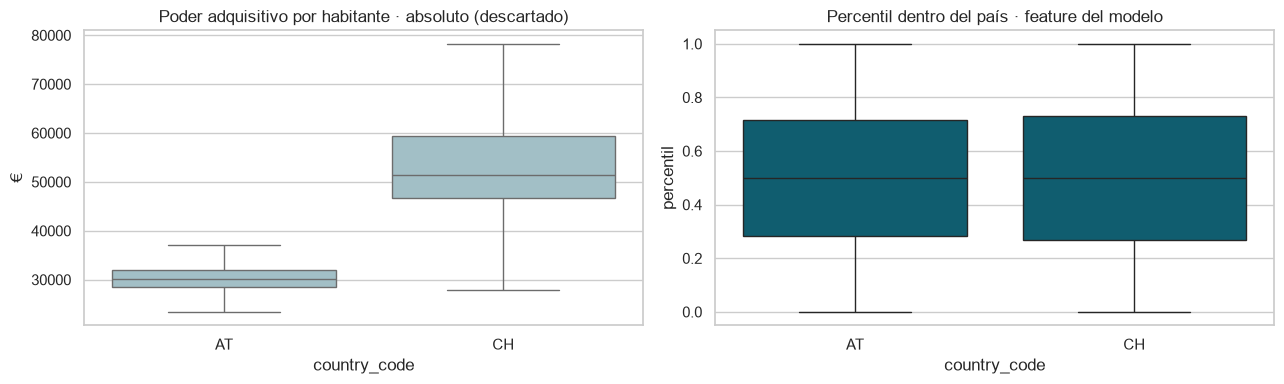
\includegraphics[width=0.85\textwidth]{r2_percentil_pais.png}
  \caption{Poder adquisitivo por habitante en euros (descartado) y como percentil dentro del país (variable del
           modelo).}
  \label{fig:percentil}
\end{figure}

\subsection{Reto 3 · Modelo K-Means}\label{sec:r3}

Se entrenó K-Means para $k=2,\dots,10$. El coeficiente de silueta se calculó sobre tres muestras aleatorias de 20.000
clientes (su coste es cuadrático), con una desviación entre muestras inferior a 0,001. La figura~\ref{fig:codo} muestra
que no hay un codo nítido (la mayor caída de inercia se produce al pasar a $k=4$, un 9,0\pct) y que la silueta alcanza
su máximo en $k=4$ (0,170), con una meseta entre $k=5$ y $k=8$ (0,132--0,138).

\begin{figure}[H]
  \centering
  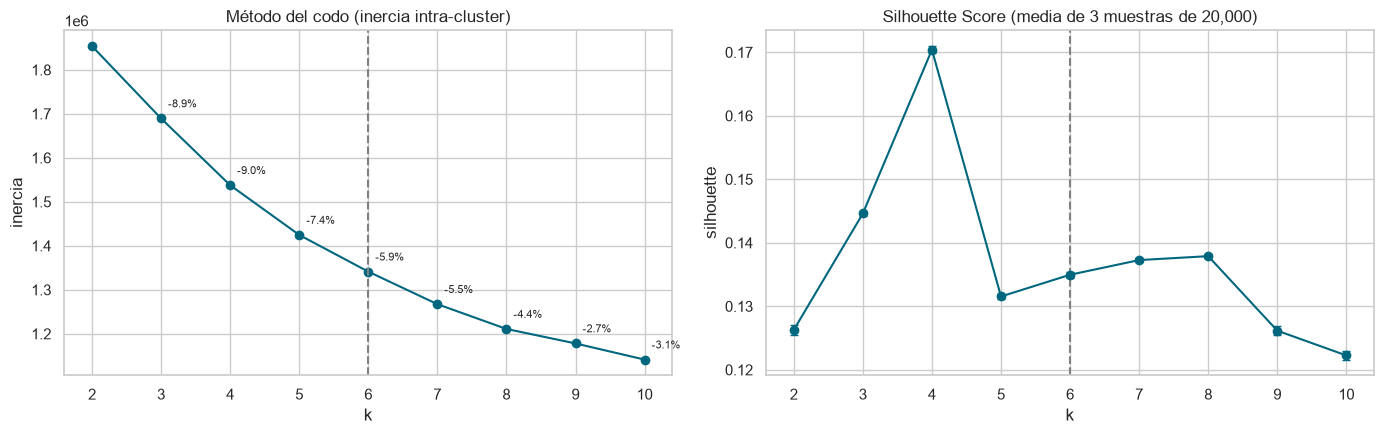
\includegraphics[width=\textwidth]{r3_codo_silhouette.png}
  \caption{Método del codo y coeficiente de silueta para $k=2,\dots,10$. La línea discontinua marca el $k$ elegido.}
  \label{fig:codo}
\end{figure}

\paragraph{Elección de $k=6$.} Con $k=4$, el modelo separa tres grupos muy marcados (multivehículo, electrificados y
furgonetas) y deja al 57\pct\ de los clientes en un único grupo genérico (figura~\ref{fig:k4k6}). Con $k=6$, ese bloque
se divide en tres grupos con uso comercial directo (clientes recientes con poco taller, clientes fieles al taller y
clientes con pocos consentimientos), el grupo más grande baja al 27\pct, la silueta se mantiene en la meseta (0,135) y
ningún grupo está dominado por un país (entre el 55\pct\ y el 74\pct\ de suizos, frente al 66\pct\ global). A partir de
$k=7$ aparece un grupo de leasing con un 86\pct\ de suizos.

\begin{figure}[H]
  \centering
  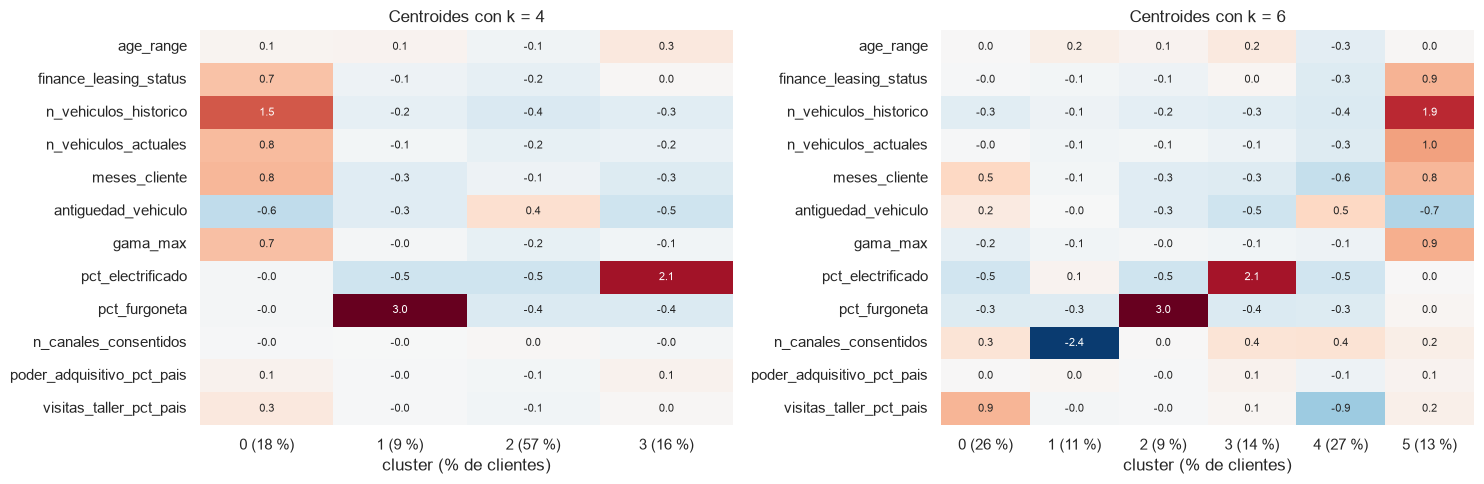
\includegraphics[width=\textwidth]{r3_k4_vs_k6.png}
  \caption{Centroides con $k=4$ y con $k=6$ (desviaciones respecto a la media).}
  \label{fig:k4k6}
\end{figure}

\paragraph{Estabilidad frente a la inicialización.} El modelo final usa 50 inicializaciones y semilla fija. Con la
primera versión del \emph{pipeline} (poder adquisitivo por hogar), diez inicializaciones producían dos soluciones
distintas según la semilla (ARI 0,61 entre ellas); con 50, todas las semillas convergen a la misma (ARI 0,997). El
apartado~\ref{sec:a3} muestra que este riesgo sigue existiendo en submuestras.

\paragraph{Silueta por grupo.} Los grupos definidos por un rasgo muy marcado son los más compactos; el grupo
multivehículo es el más difuso (silueta 0,048, con un 40\pct\ de clientes con silueta negativa), lo que motiva su
subdivisión en el Reto~4 (figura~\ref{fig:silcluster}).

\begin{figure}[H]
  \centering
  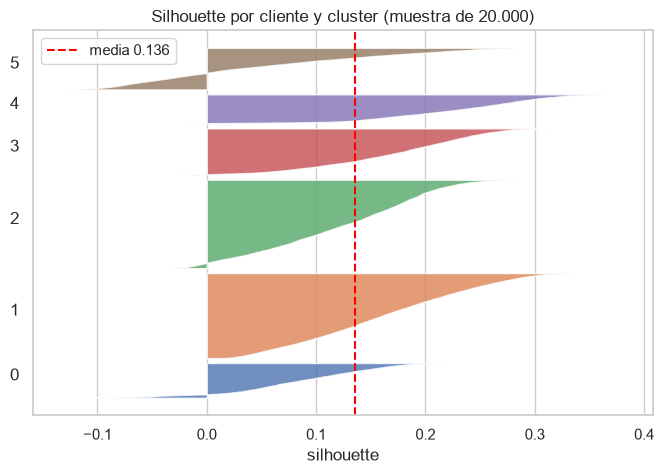
\includegraphics[width=0.6\textwidth]{r3_silhouette_cluster.png}
  \caption{Silueta por cliente y grupo (muestra de 20.000 clientes).}
  \label{fig:silcluster}
\end{figure}

\subsection{Reto 4 · Interpretación de los segmentos}\label{sec:r4}

Los nombres se asignan con reglas sobre los centroides, para que no dependan del número arbitrario de cada grupo: el de
más furgonetas es \seg{Gran Formato}, el de más electrificados \seg{Pionero Eléctrico}, el de menos canales
\seg{Contacto Solo Digital}, el de más vehículos \seg{Premium Multivehículo}, y de los dos restantes, el de más visitas al
taller es \seg{Fiel de Taller} y el de menos \seg{Recién Llegado de Ocasión}. La figura~\ref{fig:huella} muestra la
\emph{huella} de cada segmento y la tabla~\ref{tab:segmentos} los resume.

\begin{figure}[H]
  \centering
  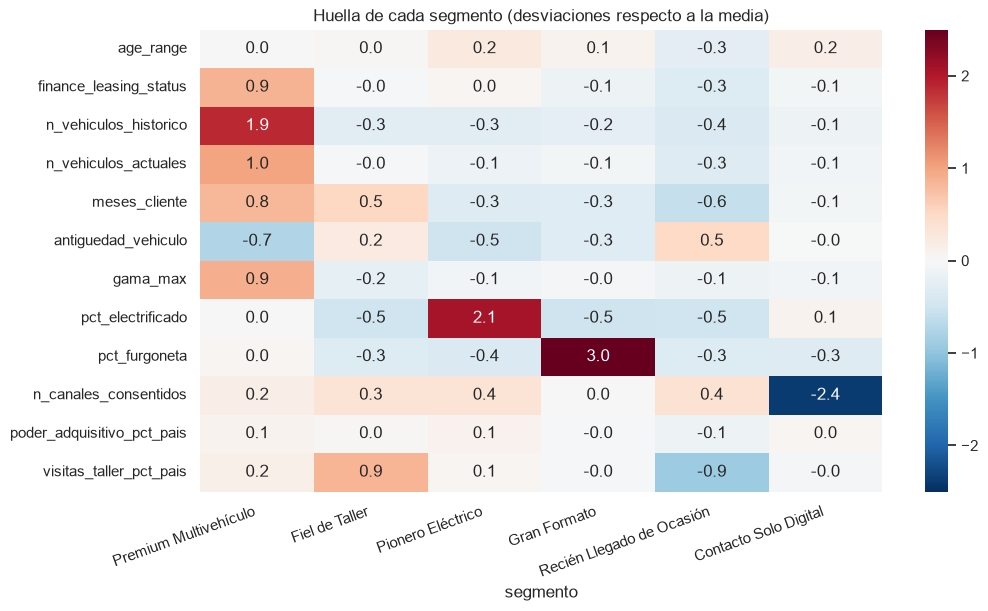
\includegraphics[width=0.85\textwidth]{r4_huella.png}
  \caption{Huella de cada segmento: diferencia respecto a la media en desviaciones estándar.}
  \label{fig:huella}
\end{figure}

\begin{table}[H]
  \centering
  \small
  \caption{Los seis segmentos.}
  \label{tab:segmentos}
  \begin{tabularx}{\textwidth}{>{\raggedright\arraybackslash}p{3.1cm}rLL}
    \toprule
    Segmento & \% & Rasgos & Prioridad comercial \\
    \midrule
    Premium Multivehículo & 12,9 & Mediana de 3 Mercedes, la mitad con 2 o más a la vez, 58,5\pct\ con leasing, coches
      de menos de 2 años, 61\pct\ gama alta, 36\pct\ con algún AMG & Retener y renovar (mayor valor) \\
    Fiel de Taller & 26,2 & Veterano (42 meses), coche compacto o medio de unos 5 años, uso del taller muy superior a
      la media & Planes de mantenimiento y renovación \\
    Pionero Eléctrico & 14,3 & 97\pct\ de vehículos híbridos enchufables o eléctricos, coches de unos 3 años, más peso
      de Austria & Gama EQ y servicios eléctricos \\
    Gran Formato & 8,8 & Furgonetas (Clase V/Vito, Sprinter); solo un 3\pct\ de relaciones de empresa & Renovación de
      furgoneta y furgonetas eléctricas \\
    Recién Llegado de Ocasión & 27,1 & Cliente más reciente (20 meses), coche de unos 6 años, apenas usa el taller,
      18\pct\ inactivos & Primer coche nuevo, captación al taller, retención \\
    Contacto Solo Digital & 10,9 & Perfil medio; el 79\pct\ solo acepta email & Recuperar consentimientos \\
    \bottomrule
  \end{tabularx}
\end{table}

\paragraph{Comprobaciones antes de poner nombres.} Comparando coches de la misma edad, \seg{Fiel de Taller} tiene más
visitas en todas las bandas de antigüedad y \seg{Recién Llegado} menos en todas: la diferencia es de comportamiento y no
de edad del coche. El 81\pct\ de \seg{Recién Llegado} tiene un coche más de un año anterior a su relación con la marca,
lo que apunta a una entrada por el mercado de ocasión; se presenta como \textbf{hipótesis}, pendiente de validar con datos
de ventas. \seg{Contacto Solo Digital} no es un grupo de clientes no contactables (el 89\pct\ acepta email), sino un
segmento de \emph{canal}. El poder adquisitivo de la zona y la forma de conducir no diferencian a ningún segmento. Por
último, un K-Means interno sobre \seg{Premium Multivehículo} separa tres subperfiles estables: \emph{Renovador en
Leasing} (50\pct), \emph{Premium al Contado} (34\pct) y \emph{Gran Cuenta / Flota} (16\pct).

\paragraph{Segmentos y datos externos.} Las zonas donde viven los segmentos se parecen mucho (figura~\ref{fig:zona}):
solo \seg{Gran Formato} vive claramente más lejos del hospital (un 18--20\pct\ más en ambos países) y, en Austria, en
zonas con más accidentes graves; \seg{Recién Llegado} es el más urbano. La incertidumbre se mide con un
\emph{bootstrap} por zonas, porque los clientes de una misma zona no son observaciones independientes. Al introducir los
indicadores de zona en el K-Means se obtienen los mismos segmentos (ARI 0,978) con peor silueta (0,102); si se les da
más peso, los segmentos pasan a ser geográficos. Por eso se usan como capa de perfilado y no como variables del modelo.

\begin{figure}[H]
  \centering
  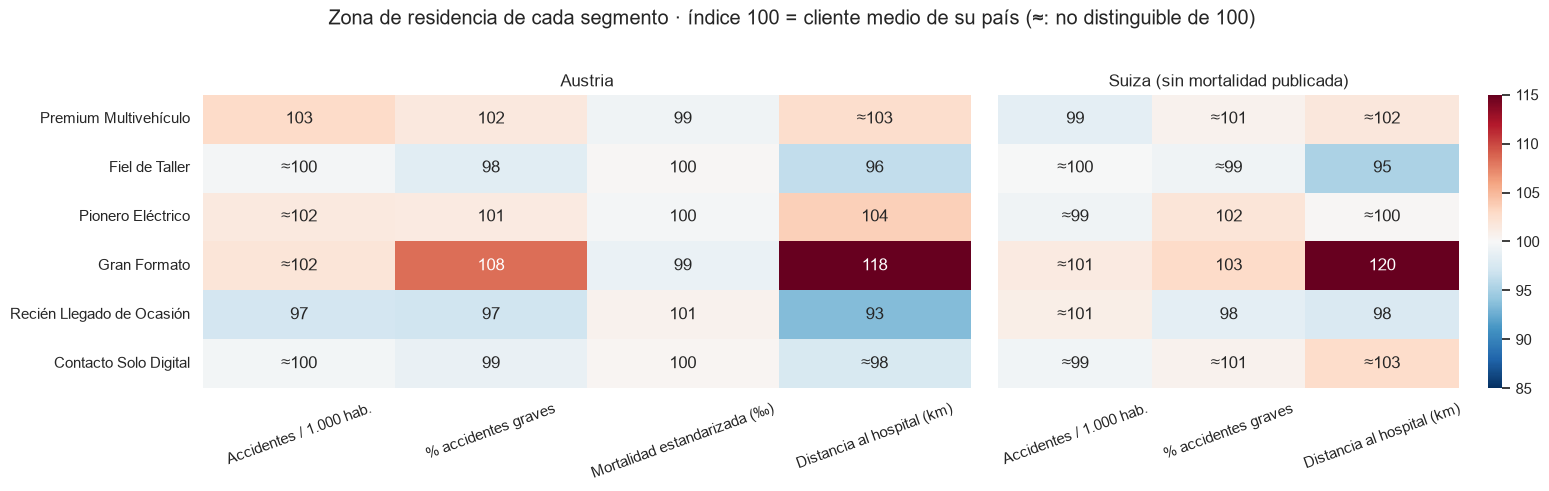
\includegraphics[width=\textwidth]{r4_zona.png}
  \caption{Zona de residencia de cada segmento (índice 100 = cliente medio de su país). El símbolo $\approx$ indica que el
           intervalo de confianza del \emph{bootstrap} por zonas incluye el 100.}
  \label{fig:zona}
\end{figure}

\paragraph{Oportunidades ocultas.} Al cruzar los segmentos con las relaciones no evidentes del Reto~1 aparecen públicos
que la etiqueta del segmento no cuenta (figura~\ref{fig:ocultas}). \seg{Premium Multivehículo} es el segmento que menos
carga sus híbridos (casi uno de cada cinco consume como un combustión) y concentra la mayoría de los hogares mixtos
(unos 1.900): es donde está el siguiente eléctrico. \seg{Pionero Eléctrico} tiene la mayor proporción de clientes con
coche nuevo que nunca han ido al taller (unos 4.300): el eléctrico necesita poco mantenimiento y la marca pierde el
contacto físico. \seg{Recién Llegado} concentra el riesgo de abandono y los perfiles incompletos. Antes de usar la señal
\emph{coche nuevo sin visitas} se comprobó que no es un artefacto de los eléctricos: entre los clientes con coche
reciente, los que no van al taller están inactivos entre 3 y 6 veces más en todos los tipos de vehículo.

\begin{figure}[H]
  \centering
  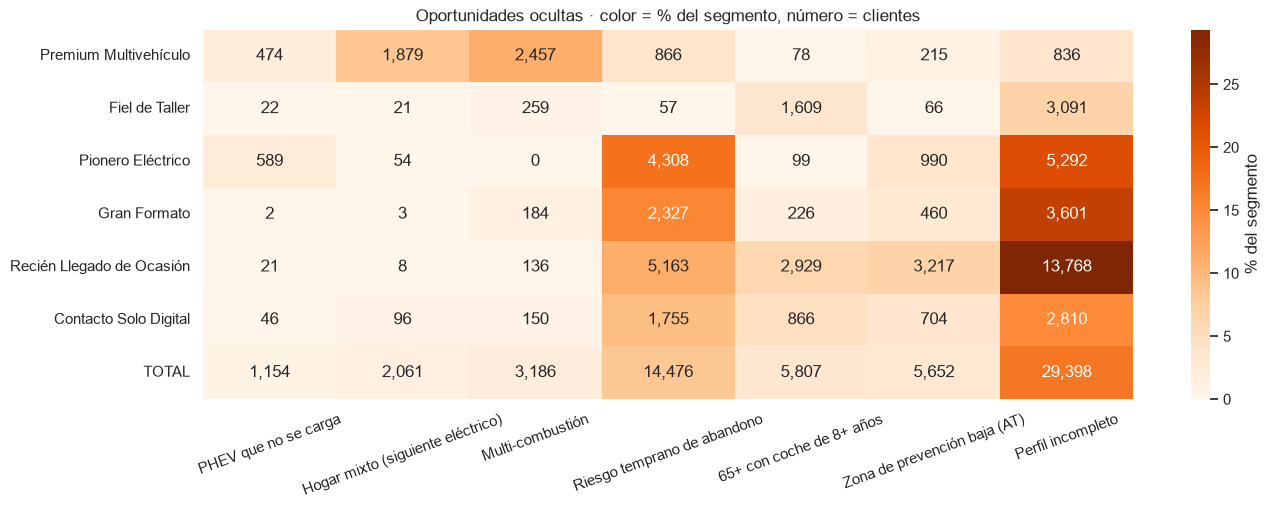
\includegraphics[width=\textwidth]{r4_ocultas.png}
  \caption{Oportunidades ocultas por segmento: el color indica el porcentaje del segmento y el número, los clientes.}
  \label{fig:ocultas}
\end{figure}

\paragraph{Ergonomía por segmento.} La figura~\ref{fig:ergo} relaciona la necesidad ergonómica esperada con el coche que
conduce cada segmento. Unos 21.000 clientes con una limitación esperada conducen un coche que no es alto; la mayor brecha
está en \seg{Recién Llegado de Ocasión} (unos 8.200) y \seg{Fiel de Taller} (unos 6.700). Para cada problema de salud se
propone un equipamiento concreto (posición alta y acceso sin llave para la limitación general; asientos con apoyo lumbar
y masaje para el dolor lumbar; cámara de 360° y asistentes de maniobra para el cervical), siempre con un mensaje de
comodidad y nunca de salud o edad.

\begin{figure}[H]
  \centering
  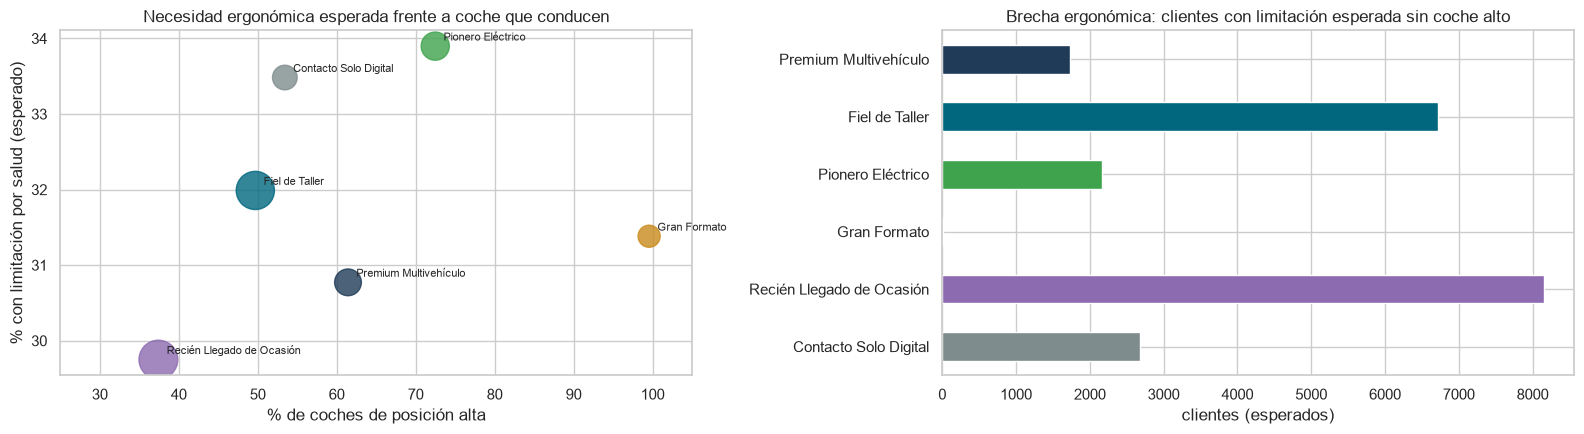
\includegraphics[width=\textwidth]{r4_ergonomia.png}
  \caption{Necesidad ergonómica esperada frente a la proporción de coches de posición alta (izquierda) y clientes con
           limitación esperada sin coche alto, por segmento (derecha).}
  \label{fig:ergo}
\end{figure}

\subsection{Avanzado 1 · Comparativa de algoritmos}\label{sec:a1}

Se compararon, con el mismo $k=6$ y las mismas variables, K-Means, GMM (estándar y regularizado), el agrupamiento
aglomerativo con tres criterios de enlace y DBSCAN (tabla~\ref{tab:comparativa}). Todas las métricas se calculan sobre la
misma muestra de 20.000 clientes.

\begin{table}[H]
  \centering
  \small
  \caption{Comparativa de algoritmos ($k=6$).}
  \label{tab:comparativa}
  \begin{tabular}{lrrrrl}
    \toprule
    Algoritmo & Silueta & Calinski-H. & Davies-B. & Grupo mayor & Estabilidad \\
    \midrule
    K-Means & 0,136 & \textbf{2.205} & \textbf{1,89} & \textbf{27\pct} & ARI 0,997 entre semillas \\
    GMM estándar & 0,114 & 1.727 & 2,62 & 46\pct & ARI 0,47--0,72 entre semillas \\
    GMM regularizado & 0,139 & 1.953 & 2,01 & 38\pct & Sensible a la regularización \\
    Aglomerativo (Ward) & 0,150 & 1.901 & 1,95 & 40\pct & ARI 0,51--0,82 entre muestras \\
    Aglomerativo (\emph{average}) & 0,155 & 296 & 1,41 & 95\pct & Degenerado \\
    \bottomrule
  \end{tabular}
\end{table}

Los hallazgos principales son tres. Primero, el GMM \textbf{degenera} con variables casi discretas: varias varianzas caen
al mínimo permitido y asigna a todos los clientes con probabilidad 1. Segundo, el aglomerativo no cabe en memoria con
toda la base (unos 120~GB) y depende de la muestra; su enlace \emph{average} obtiene la mejor silueta del reto
mientras mete al 95\pct\ de los clientes en un solo grupo, un ejemplo claro de que una métrica alta no garantiza una
segmentación útil (figura~\ref{fig:a1}). Tercero, DBSCAN no encuentra zonas densas separadas: con un radio pequeño, la
mayoría de los clientes es ruido, y con uno grande, un grupo absorbe al 65--84\pct. Segmento a segmento, \seg{Gran
Formato} y \seg{Pionero Eléctrico} se reproducen con todos los métodos, mientras que \seg{Fiel de Taller} y \seg{Recién
Llegado} se fusionan en el grupo grande de los demás algoritmos: son un corte útil dentro de un continuo. La conclusión es
que \textbf{K-Means es el algoritmo más adecuado}: el más equilibrado, el más estable y el único que usa toda la base.

\begin{figure}[H]
  \centering
  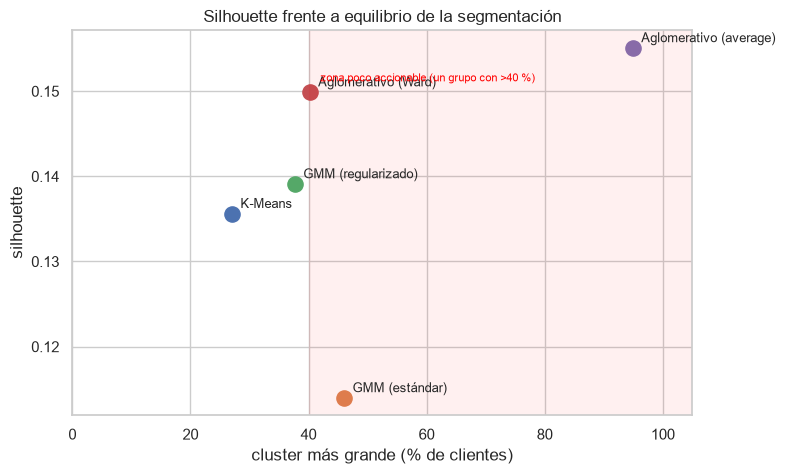
\includegraphics[width=0.7\textwidth]{a1_silhouette_equilibrio.png}
  \caption{Silueta frente al tamaño del grupo más grande. Las mejoras de silueta de otros algoritmos se obtienen a costa
           de un grupo gigante.}
  \label{fig:a1}
\end{figure}

\subsection{Avanzado 2 · Reducción de dimensionalidad}\label{sec:a2}

La varianza está muy repartida (figura~\ref{fig:varianza}): la primera componente recoge el 18,1\pct\ y la segunda el
12,4\pct, de modo que el plano PC1--PC2 solo muestra el 30,5\pct\ de la información y hacen falta ocho componentes para
superar el 80\pct. PC1 representa la \emph{intensidad de la relación con la marca} (muchos vehículos, más meses como
cliente, leasing, gama alta y coches nuevos) y PC2 opone al \emph{cliente veterano con un coche de combustión antiguo}
al \emph{cliente reciente con un coche electrificado}.

\begin{figure}[H]
  \centering
  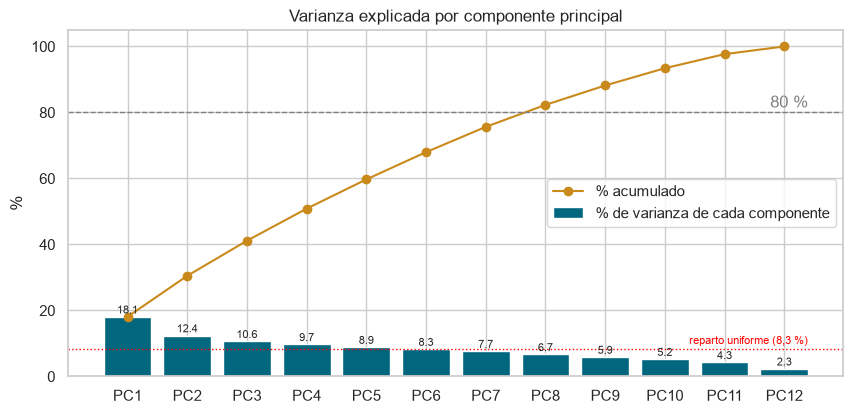
\includegraphics[width=0.7\textwidth]{a2_varianza.png}
  \caption{Varianza explicada por componente principal y varianza acumulada.}
  \label{fig:varianza}
\end{figure}

En el plano PC1--PC2 (figura~\ref{fig:scatter}) solo \seg{Premium Multivehículo} y \seg{Pionero Eléctrico} se separan
con claridad; \seg{Gran Formato} y \seg{Contacto Solo Digital} se definen en PC5 y PC6, que no aparecen en el gráfico,
y se ven claramente separados al dibujar esas componentes. La silueta medida solo con dos componentes es de 0,070, la
mitad que con las doce variables; con seis componentes sube a 0,187, por encima del modelo completo, porque las últimas
componentes añaden sobre todo ruido. \textbf{En 2D los segmentos no son visualmente separables en su conjunto, pero sí
lo son en el espacio completo}: el gráfico bidimensional infravalora la separación.

\begin{figure}[H]
  \centering
  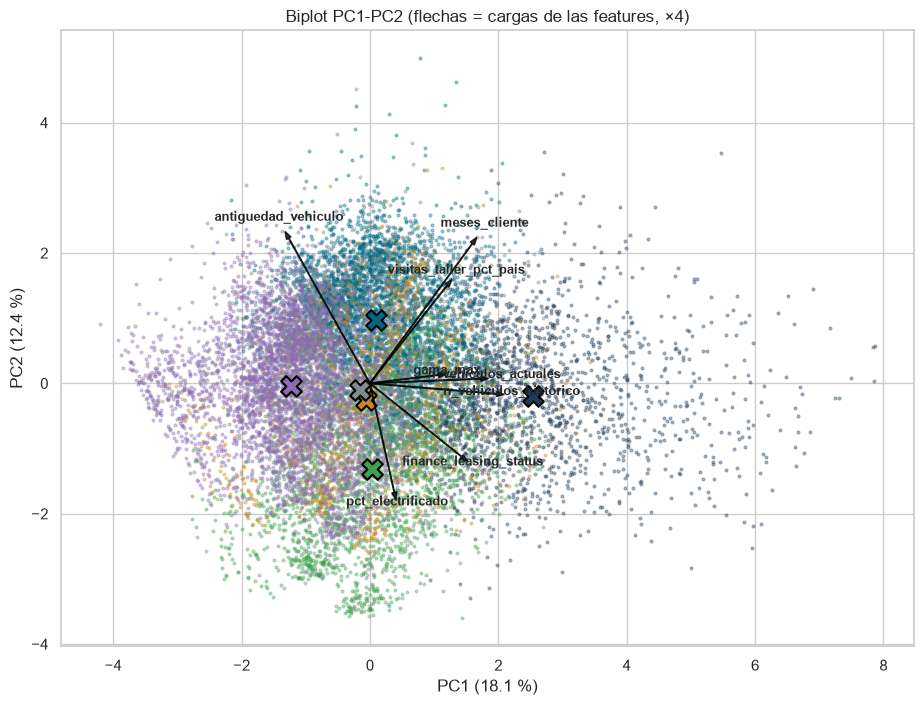
\includegraphics[width=0.75\textwidth]{a2_scatter.png}
  \caption{Biplot PC1--PC2: clientes coloreados por segmento, centroides (cruces) y cargas de las variables (flechas).}
  \label{fig:scatter}
\end{figure}

\subsection{Avanzado 3 · Estabilidad con Jackknife Clustering}\label{sec:a3}

Se generaron 20 submuestras excluyendo cada vez el 20\pct\ de los clientes (y otras 20 con el 10\pct). En cada una se
re-entrenó \textbf{el \emph{pipeline} completo} (percentiles, escalado, imputación y K-Means con 50 inicializaciones),
excluyendo \textbf{clientes enteros y no filas}, para no alterar los agregados de los que se quedan. Las etiquetas se
alinearon con la referencia mediante el algoritmo húngaro, y se usaron también medidas que no dependen del
emparejamiento: el ARI y la Jaccard por grupo de \textcite{hennig2007}.

\paragraph{Resultados.} Cada ejecución reproduce la segmentación con un ARI medio de 0,995 y un 99,8\pct\ de clientes en
el mismo segmento (figura~\ref{fig:a3ari}); un control que solo cambia la semilla da casi lo mismo (0,997), así que la
variación restante procede de la inicialización y no de los datos. El \textbf{99,1\pct\ de los clientes} cae siempre en
el mismo segmento y todos los segmentos superan con holgura el umbral de estabilidad (Jaccard media $\ge 0{,}99$).
Los más sólidos son \seg{Gran Formato} y \seg{Pionero Eléctrico}; los menos, \seg{Premium Multivehículo} y \seg{Fiel de
Taller} (1,3--1,5\pct\ de clientes que cambian alguna vez). Los 1.555 clientes que cambian están todos en el 10\pct\ más
cercano a una frontera y saltan hacia su segundo segmento más próximo, sobre todo entre \seg{Fiel de Taller} y
\seg{Recién Llegado} (figura~\ref{fig:a3saltos}).

\begin{figure}[H]
  \centering
  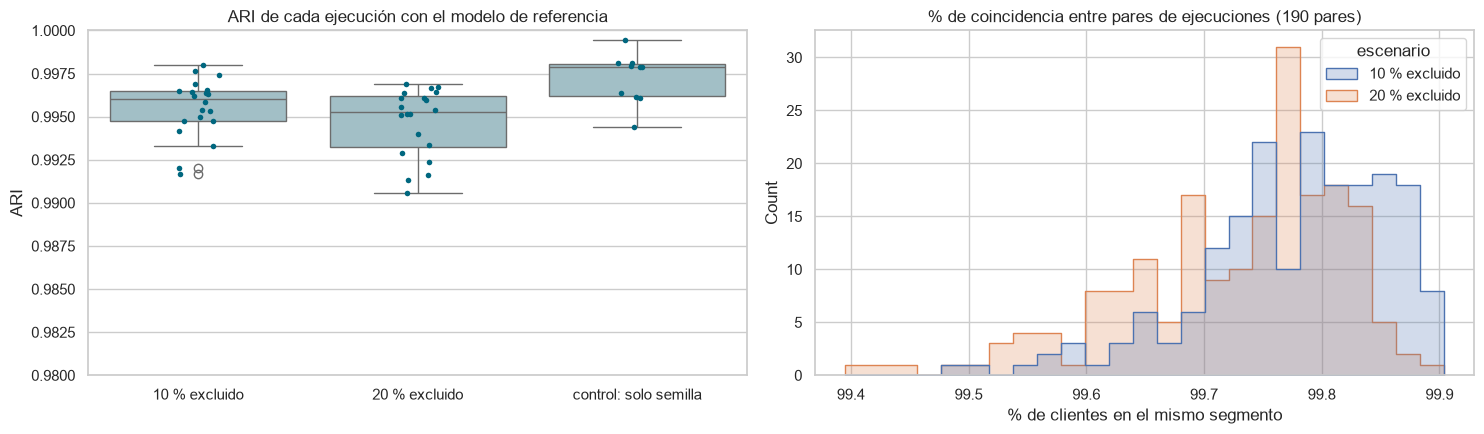
\includegraphics[width=\textwidth]{a3_ari.png}
  \caption{ARI de cada ejecución con el modelo de referencia (izquierda) y coincidencia entre pares de ejecuciones
           (derecha).}
  \label{fig:a3ari}
\end{figure}

\begin{figure}[H]
  \centering
  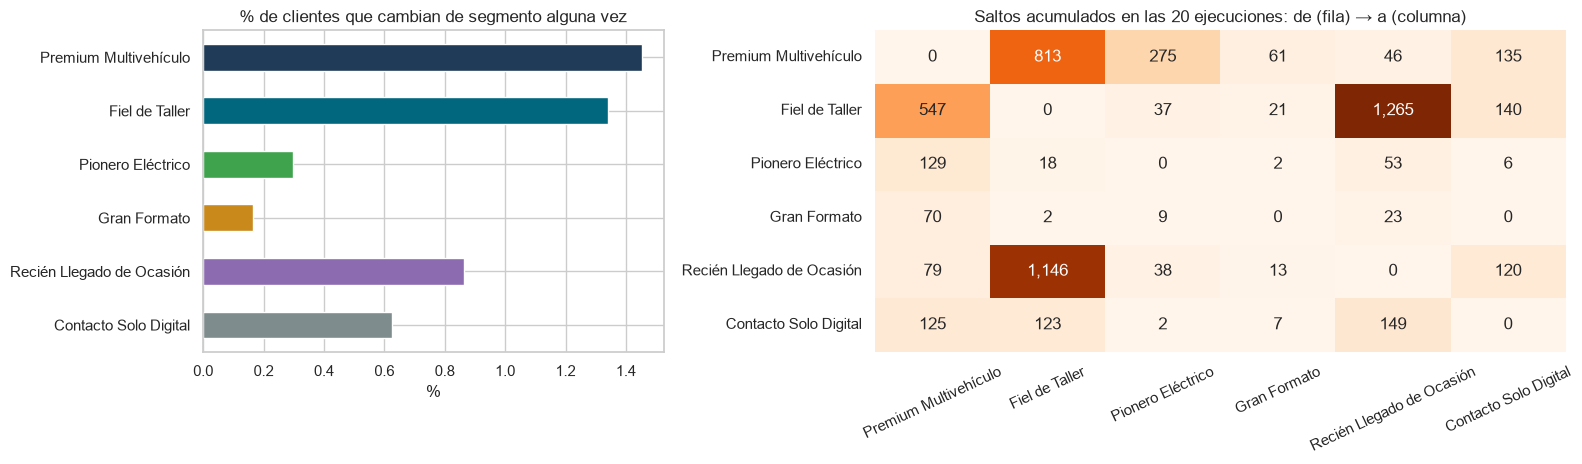
\includegraphics[width=\textwidth]{a3_saltos.png}
  \caption{Porcentaje de clientes que cambian de segmento alguna vez (izquierda) y saltos acumulados en las 20
           ejecuciones (derecha).}
  \label{fig:a3saltos}
\end{figure}

\paragraph{¿Estructura real o efecto del algoritmo?} Como K-Means siempre devuelve $k$ grupos, se repitió el
experimento con un \textbf{modelo nulo} (cada columna barajada por separado, lo que destruye cualquier relación entre
variables) y con exclusiones mucho mayores (figura~\ref{fig:a3nulo}). Los datos reales mantienen la segmentación hasta
excluir el 70\pct\ de los clientes (ARI $\ge 0{,}98$), mientras que los datos barajados se quedan en torno a 0,7: la
estabilidad refleja \textbf{estructura real}.

\begin{figure}[H]
  \centering
  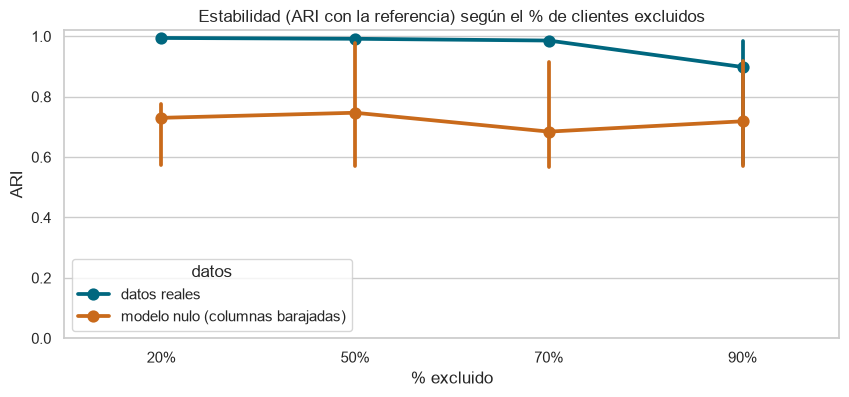
\includegraphics[width=0.75\textwidth]{a3_estres_nulo.png}
  \caption{Estabilidad según el porcentaje de clientes excluidos, con los datos reales y con el modelo nulo.}
  \label{fig:a3nulo}
\end{figure}

\paragraph{La fragilidad escondida.} Con diez inicializaciones, dos de cada seis submuestras dieron una segmentación
distinta (ARI 0,61). Existe una \textbf{solución alternativa casi empatada} (inercia solo un 0,15\pct\ mayor) en la que
\seg{Contacto Solo Digital} desaparece y surge un segmento de \textbf{leasing activo} (figura~\ref{fig:a3alt}). Con una
sola inicialización, K-Means llega el doble de veces a la alternativa que a la solución de referencia; con 50, la
probabilidad de no encontrar la mejor es prácticamente nula. La estabilidad de la segmentación depende, por tanto, de
optimizar bien, y \seg{Contacto Solo Digital} es el segmento estructuralmente más frágil. Por último, la estabilidad
según $k$ confirma que $k=6$ es una elección estable, como cualquier $k$ entre 3 y 8; solo $k=9$ baja (0,91).

\begin{figure}[H]
  \centering
  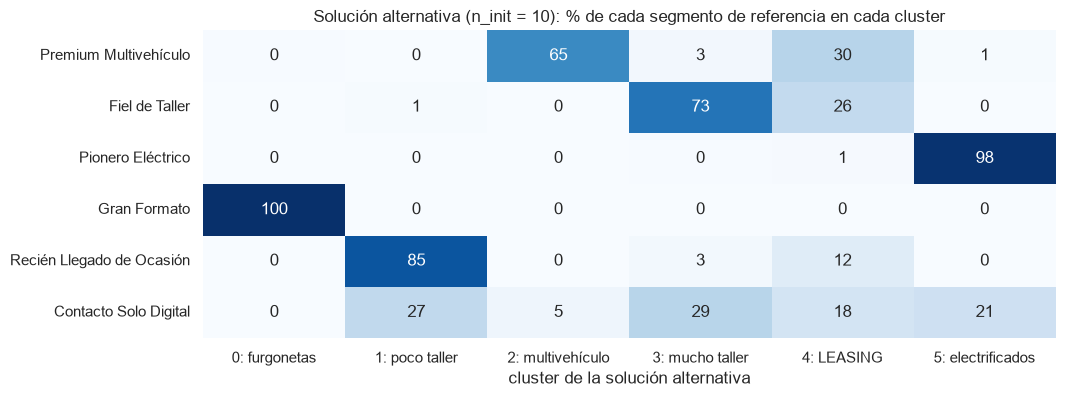
\includegraphics[width=0.85\textwidth]{a3_alternativa.png}
  \caption{Solución alternativa encontrada con diez inicializaciones: porcentaje de cada segmento de referencia en cada
           grupo.}
  \label{fig:a3alt}
\end{figure}

\subsection{Extra · Salud y seguridad vial por zona}\label{sec:extra}

La construcción de los indicadores de zona exigió resolver varios detalles: extraer del informe en PDF de Statistik
Austria las tablas por distrito con un analizador que valida las sumas (los 116 distritos suman exactamente los 37.825
accidentes oficiales); tratar Viena como un único municipio en unas fuentes y como 23 distritos en otras; asignar los
códigos postales compartidos por varios municipios; excluir autopistas (inflarían la tasa de los pueblos de paso);
excluir los años de la COVID en la mortalidad, y no calcular tasas en municipios suizos de menos de 1.000 habitantes.
La población de cada código postal procede del propio CSV y suma prácticamente la población oficial de ambos países.

La figura~\ref{fig:extra} resume las correlaciones entre zonas. En Austria (115 distritos), los distritos con más
mortalidad tienen clientes con coches más antiguos (+0,35) y más \seg{Recién Llegado} (+0,45); los de más accidentes
graves, más \seg{Gran Formato} (+0,62) y más clientes de 65 años o más (+0,36), el perfil rural. En Suiza, las
relaciones son débiles. Con ello se cuantificaron públicos concretos (por ejemplo, unos 14.600 clientes en zonas de
alta siniestralidad con un coche anterior a julio de 2024, fecha de entrada en vigor de los asistentes obligatorios del
Reglamento (UE) 2019/2144; \cite{gsr2019}) y acciones Mercedes-Benz asociadas (renovación con asistentes de seguridad,
llamada de emergencia, tracción 4MATIC).

\begin{figure}[H]
  \centering
  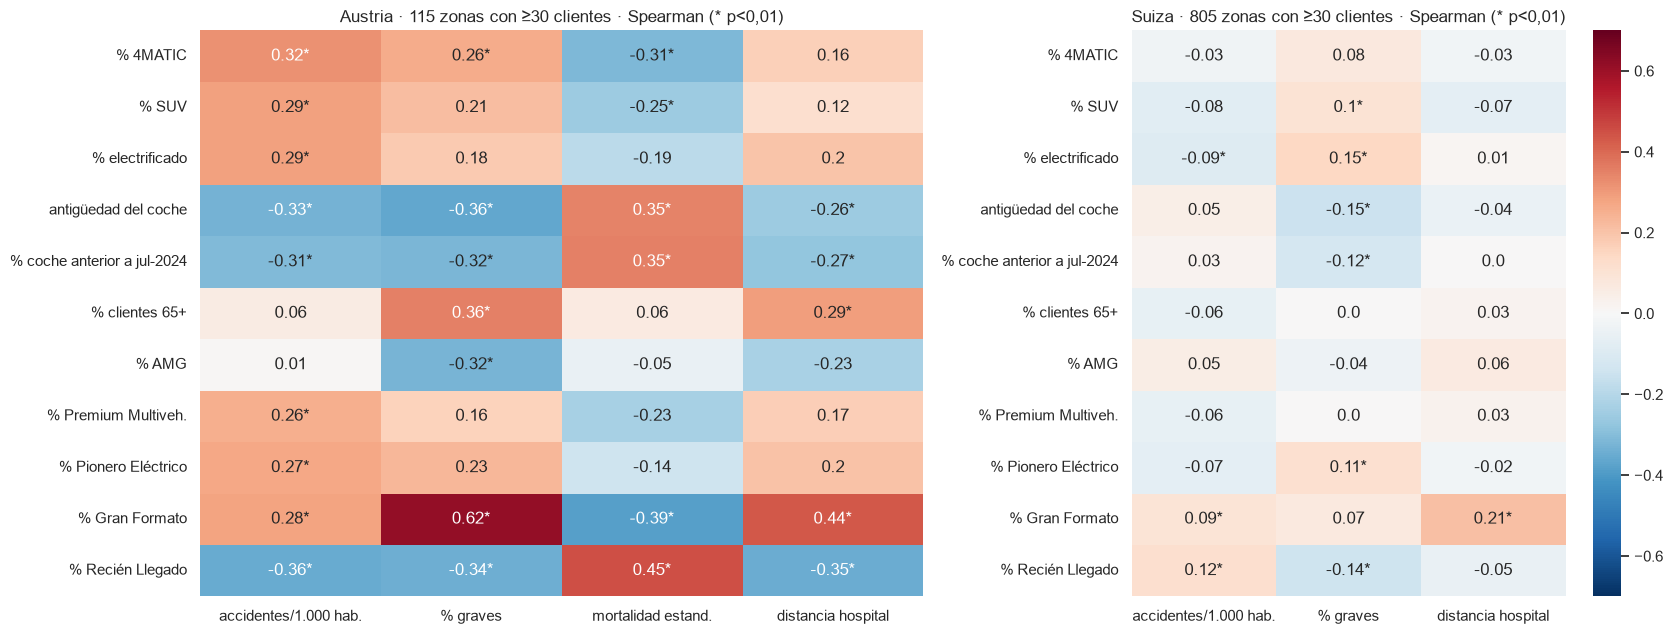
\includegraphics[width=\textwidth]{ex_correlaciones.png}
  \caption{Correlación de Spearman entre los indicadores de zona y el perfil de los clientes, en Austria y Suiza
           (* $p<0{,}01$).}
  \label{fig:extra}
\end{figure}

% ===========================================================================
\section{Aclaraciones}\label{sec:aclaraciones}
% ===========================================================================

Esta sección responde a las preguntas que con más frecuencia surgen al leer los resultados.

\paragraph{¿Un coeficiente de silueta de 0,135 invalida la segmentación?} No. La silueta mide lo separados que están los
grupos, y en una base de clientes las variables forman un \emph{continuo} más que grupos aislados. En comprobaciones
complementarias, los mismos datos con las columnas barajadas dan una silueta de aproximadamente 0,10, y el ruido puro,
de aproximadamente 0,05; con solo las cinco variables que definen los segmentos, la silueta se acerca a 0,39. Es decir,
hay estructura real, diluida por variables que aportan matices pero no separan. Lo decisivo para marketing es que los
segmentos sean distintos, estables (sección~\ref{sec:a3}) y accionables, no que estén aislados.

\paragraph{¿Por qué $k=6$ si la silueta máxima está en $k=4$?} Porque $k=4$ deja al 57\pct\ de los clientes en un grupo
genérico, sin estrategia propia. $k=6$ se mantiene en la meseta de la silueta, reparte toda la base en grupos
accionables y es igual de estable (sección~\ref{sec:a3}). La elección combina el criterio estadístico con el de negocio,
como recomienda la literatura \parencite{wedel2000}.

\paragraph{¿Por qué percentiles dentro de cada país?} Porque en euros cualquier suizo es \enquote{rico} frente a un
austriaco, y las visitas al taller se registran de forma distinta en cada mercado. Sin esta corrección, el modelo
habría separado países en lugar de tipos de cliente, algo que ya se sabe y que no ayuda a hacer campañas.

\paragraph{¿Por qué la telemetría no entra en el modelo?} Porque falta de forma estructural: no existe para los
eléctricos, para la mayoría de los roles no propietarios ni para los coches anteriores a 2016. Imputarla inventaría
conducción, y un indicador de \enquote{tiene telemetría} separaría eléctricos y coches antiguos en lugar de tipos de
cliente. Se usa, con esa advertencia, para perfilar y validar.

\paragraph{¿Por qué el poder adquisitivo por habitante y no por hogar?} Porque el valor por hogar crece con el tamaño
del hogar, que es mayor en las zonas rurales: medía en parte ruralidad, no riqueza. El cambio apenas modificó los
segmentos (ARI 0,98), pero hizo desaparecer un falso segmento \enquote{urbano y de menor poder adquisitivo} que aparecía
con $k=8$.

\paragraph{¿Por qué los datos externos no son variables del modelo?} Porque describen a los vecinos y no al cliente
(todos los clientes de un distrito comparten el valor), porque la mortalidad solo existe en Austria y porque, al
probarlo, no cambian los segmentos con su peso natural y los vuelven geográficos si se les da más peso.

\paragraph{¿Las correlaciones entre zonas demuestran causas?} No. Son relaciones entre zonas, sujetas a la falacia
ecológica \parencite{robinson1950}, y muchas se explican por la diferencia entre lo urbano y lo rural. Se controlan con
correlaciones parciales y se presentan como hipótesis que orientan dónde y qué comunicar.

\paragraph{¿Se usan datos de salud de los clientes?} No. A cada cliente se le asigna la prevalencia oficial de su país,
edad y sexo: es una probabilidad esperada, útil para estimar cuántos clientes de un grupo tienen probablemente un
problema y qué equipamiento conviene destacar, pero que no dice nada de una persona concreta. Los mensajes comerciales
derivados deben hablar de comodidad, nunca de salud ni de edad \parencite{rgpd2016}.

\paragraph{¿Es seguro que \seg{Recién Llegado de Ocasión} compró un coche usado?} No. La antigüedad como cliente cuenta
desde la primera conexión de un coche, no desde la compra, por lo que otra explicación posible es una activación tardía
de los servicios conectados. Debe validarse con datos de ventas antes de basar campañas en ello.

\paragraph{¿Qué es exactamente un \enquote{índice 100}, un ARI o una Jaccard?} El índice 100 compara un segmento con el
cliente medio de su país (118 significa un 18\pct\ más). El ARI mide el parecido entre dos agrupaciones (1 = idénticas, 0
= como al azar) sin depender de cómo se numeren los grupos. La Jaccard mide el solapamiento entre dos grupos (clientes en
común entre clientes en total).

\paragraph{¿Cómo se garantiza la reproducibilidad?} Toda la preparación está en \texttt{features.py}; el modelo usa
siempre 50 inicializaciones y la semilla 42; los notebooks se ejecutan de principio a fin, y las tablas externas ya
resumidas (\texttt{datos\_externos\_por\_cp.csv} y \texttt{datos\_salud\_edad\_sexo.csv}) están en el repositorio.

% ===========================================================================
\section{Conclusiones}\label{sec:conclusiones}
% ===========================================================================

\begin{enumerate}
  \item \textbf{La calidad del dato condiciona el resultado.} La granularidad cliente--vehículo, los nulos estructurales
        de la telemetría, la diferencia de registro de las visitas entre países y el sesgo del poder adquisitivo por
        hogar habrían producido segmentos erróneos si no se hubieran detectado y corregido.
  \item \textbf{Seis segmentos accionables.} \seg{Premium Multivehículo}, \seg{Fiel de Taller}, \seg{Pionero Eléctrico},
        \seg{Gran Formato}, \seg{Recién Llegado de Ocasión} y \seg{Contacto Solo Digital} cubren toda la base, ninguno
        está dominado por un país y cada uno tiene una estrategia propia.
  \item \textbf{K-Means es el algoritmo adecuado} para estos datos: más equilibrado y estable que GMM, el aglomerativo o
        DBSCAN, y el único que usa toda la base sin muestrear.
  \item \textbf{La segmentación es robusta}: el 99,1\pct\ de los clientes cae siempre en el mismo segmento al excluir un
        20\pct\ de la base, y la estructura no aparece en datos sin relación entre variables. Su punto débil es una
        solución alternativa casi empatada, que se evita con 50 inicializaciones.
  \item \textbf{Los segmentos se solapan en sus fronteras}, como muestran la silueta, el PCA y el jackknife. Los
        clientes que cambian están siempre en la frontera y saltan hacia su segundo segmento más cercano.
  \item \textbf{Los datos externos aportan contexto, no segmentos.} Permiten validar la telemetría, detectar sesgos y
        priorizar dentro de cada segmento públicos de seguridad vial y de ergonomía, siempre con un uso responsable.
  \item \textbf{Hay oportunidades que no se ven en las etiquetas}: los híbridos que no se cargan, el siguiente eléctrico
        en los hogares mixtos, la alerta de abandono \enquote{coche nuevo sin visita al taller} y la brecha ergonómica de
        unos 21.000 clientes.
\end{enumerate}

% ===========================================================================
\section{Líneas futuras}\label{sec:futuro}
% ===========================================================================

\begin{itemize}
  \item \textbf{Validar las hipótesis con datos internos adicionales}: registros de ventas (nuevo, usado, concesionario)
        para confirmar el origen de \seg{Recién Llegado de Ocasión}, y registros de siniestros para el programa posterior
        al siniestro.
  \item \textbf{Explorar una segmentación por leasing.} El Avanzado~3 muestra que el leasing es una dimensión casi tan
        fuerte como el canal; podría convertirse en segmento, con el canal como capa transversal de filtrado.
  \item \textbf{Modelo supervisado de abandono}, con la señal \enquote{coche nuevo sin visita al taller} como variable
        principal, validado sobre clientes que dejen de estar conectados en el futuro.
  \item \textbf{Seguimiento de la estabilidad en producción}: re-entrenar periódicamente, comparar con el ARI y vigilar
        el desplazamiento de los datos (por ejemplo, el crecimiento de los eléctricos).
  \item \textbf{Algoritmos y espacios alternativos}: K-Means sobre las primeras cinco o seis componentes principales,
        HDBSCAN o modelos de clases latentes para variables mixtas.
  \item \textbf{Mejores datos externos}: salud musculoesquelética por edad y sexo en Suiza (encuesta suiza de salud),
        distancias por carretera en lugar de en línea recta e indicadores a nivel de cantón.
  \item \textbf{Medir el impacto}: pruebas A/B de las campañas propuestas (renovación por seguridad, ergonomía, carga de
        híbridos) para estimar su efecto real sobre la conversión y la retención.
  \item \textbf{Datos con consentimiento}: preferencias de confort o de accesibilidad declaradas por el propio cliente,
        que permitirían pasar de probabilidades esperadas a necesidades reales.
\end{itemize}

% ===========================================================================
\printbibliography[heading=bibintoc,title={Bibliografía}]

\end{document}
